% !TEX encoding = utf8
\documentclass[a4paper,titlepage,11pt,floatssmall]{mwrep}
\usepackage[left=2.5cm,right=2.5cm,top=2.5cm,bottom=2.5cm]{geometry}
\usepackage[T1]{fontenc}
\usepackage{polski}
\usepackage[utf8]{inputenc}

% Pakiety matematyczne
\usepackage{amsmath}
\usepackage{amsfonts}
\usepackage{amssymb}

% Pakiety graficzne i inne
\usepackage{graphicx}
\usepackage{float}
\usepackage{placeins}
\usepackage{url}
\usepackage{rotating}
\usepackage{xcolor}
\usepackage{colortbl}
\usepackage{enumitem}

% Pakiet do jednostek i liczb
\usepackage{siunitx}
\sisetup{
    detect-weight,
    range-units=single,
    output-decimal-marker={,},
    exponent-product=\cdot,
    per-mode=symbol,
    table-number-alignment = center,
    table-text-alignment = center
}

% Pakiet do listingu kodu
\usepackage{listings}
\usepackage{matlab-prettifier}

\definecolor{szary}{rgb}{0.95,0.95,0.95}

% Ustawienia globalne dla listings (dla polskich znaków i tła)
\lstset{
    literate={ą}{{\k a}}1 {Ą}{{\k A}}1 {ę}{{\k e}}1 {Ę}{{\k E}}1 {ó}{{\' o}}1 {Ó}{{\' O}}1
            {ś}{{\' s}}1 {Ś}{{\' S}}1 {ł}{{\l}}1 {Ł}{{\L}}1 {ż}{{\. z}}1 {Ż}{{\. Z}}1
            {ź}{{\' z}}1 {Ź}{{\' Z}}1 {ć}{{\' c}}1 {Ć}{{\' C}}1 {ń}{{\' n}}1 {Ń}{{\' N}}1,
    showstringspaces=false,
    backgroundcolor=\color{szary},
    breaklines=true,
    basicstyle=\footnotesize\ttfamily,
    captionpos=b
}

% Definicja stylu dla kodu MATLAB
\lstdefinestyle{custommatlab}{
    style=Matlab-editor,
    literate={ą}{{\k a}}1 {Ą}{{\k A}}1 {ę}{{\k e}}1 {Ę}{{\k E}}1 {ó}{{\' o}}1 {Ó}{{\' O}}1
            {ś}{{\' s}}1 {Ś}{{\' S}}1 {ł}{{\l}}1 {Ł}{{\L}}1 {ż}{{\. z}}1 {Ż}{{\. Z}}1
            {ź}{{\' z}}1 {Ź}{{\' Z}}1 {ć}{{\' c}}1 {Ć}{{\' C}}1 {ń}{{\' n}}1 {Ń}{{\' N}}1,
    backgroundcolor=\color{szary},
    breaklines=true,
    basicstyle=\footnotesize\ttfamily,
    captionpos=b
}

% Polskie nazwy dla rysunków i tabel
\def\figurename{Rys.}
\def\tablename{Tab.}
\def\lstlistingname{Listing}

% Poprawki do składu obiektów pływających
\setcounter{topnumber}{2}
\setcounter{bottomnumber}{2}
\setcounter{totalnumber}{4}
\renewcommand{\textfraction}{0.07}
\renewcommand{\topfraction}{0.9}
\renewcommand{\bottomfraction}{0.8}
\renewcommand{\floatpagefraction}{0.7}


% --- Dane do strony tytułowej ---
\title{\bf Sprawozdanie z laboratorium \\ Sterowanie Procesami \\ Temat: Regulatory predykcyjne}
\author{Jakub Szubzda}
\date{\today}

% --- Definicja strony tytułowej ---
\makeatletter
\renewcommand{\maketitle}{\begin{titlepage}
\begin{center}{\LARGE {\bf
Wydział Elektroniki i~Technik Informacyjnych}}\\
\vspace{0.4cm}
{\LARGE {\bf Politechnika Warszawska}}\\
\vspace{0.3cm}
\end{center}
\vspace{5cm}
\begin{center}
{\bf \LARGE Przedmiot: Sterowanie procesami \vskip 0.1cm}
\end{center}
\vspace{1cm}
\begin{center}
{\bf \LARGE \@title \vskip 0.1cm}
\end{center}
\vspace{2cm}
\begin{center}
{\bf \Large Autor: \@author \par}
\end{center}
\vspace*{\stretch{6}}
\begin{center}
\bf{\large{Warszawa, \@date\vskip 0.1cm}}
\end{center}
\end{titlepage}
}
\makeatother

\begin{document}
\frenchspacing
\pagestyle{uheadings}

\maketitle

\tableofcontents

\chapter{Wstęp}

Celem projektu laboratoryjnego było zapoznanie się z~regulatorami predykcyjnymi DMC (Dynamic Matrix Control) i~GPC (Generalized Predictive Control) oraz porównanie ich działania z~klasycznym regulatorem PID. Wykonano analizę obiektu inercyjnego drugiego rzędu z~opóźnieniem, zaprojektowano dla niego regulatory predykcyjne oraz przeprowadzono symulacje w~środowisku MATLAB/Simulink.

W ramach projektu zrealizowano następujące zadania:
\begin{enumerate}
    \item Analiza transmitancji obiektu oraz jej reprezentacja w~postaci dyskretnej
    \item Wyprowadzenie równania różnicowego na podstawie transmitancji dyskretnej
    \item Strojenie regulatora PID metodą Zieglera-Nicholsa
    \item Synteza i~badanie regulatora DMC (wpływ horyzontu predykcji, horyzontu sterowania oraz współczynnika kary za sterowanie)
    \item Porównanie regulatorów DMC i~PID
    \item Porównanie regulatorów DMC i~GPC
    \item Badanie obszarów stabilności regulatorów PID, DMC i~GPC
\end{enumerate}

Projekt pozwolił na praktyczne poznanie zalet i~ograniczeń regulatorów predykcyjnych oraz nabycie umiejętności doboru ich parametrów.

\chapter{Zadania projektowe}

\section{Analiza transmitancji obiektu}

Obiektem badań był układ inercyjny drugiego rzędu z~opóźnieniem, opisany transmitancją ciągłą:
\begin{equation}
    G(s) = \frac{K_o e^{-T_o s}}{(T_1 s + 1)(T_2 s + 1)}
\end{equation}

gdzie:
\begin{itemize}
    \item $K_o = 4,7$ - współczynnik wzmocnienia statycznego
    \item $T_o = 5$ s - opóźnienie transportowe
    \item $T_1 = 1,92$ s - pierwsza stała czasowa
    \item $T_2 = 4,96$ s - druga stała czasowa
\end{itemize}

Po podstawieniu wartości parametrów uzyskano transmitancję ciągłą w~postaci:
\begin{equation}
    G(s) = e^{-5s} \cdot \frac{4,7}{9,523s^2 + 6,88s + 1}
\end{equation}

Transmitancja dyskretna została wyznaczona za pomocą funkcji \texttt{c2d(G,Tp,'zoh')} w~środowisku MATLAB, z~okresem próbkowania $T_p = 0,5$ s. Uzyskano następującą postać:
\begin{equation}
    G(z) = z^{-10} \cdot \frac{0,05477z + 0,04856}{z^2 - 1,675z + 0,6968}
\end{equation}

Współczynniki wzmocnienia statycznego dla obu transmitancji są równe $K_s = K_z = 4,7$, co potwierdza poprawność przekształcenia z postaci ciągłej na dyskretną.

\begin{figure}[H]
    \centering
    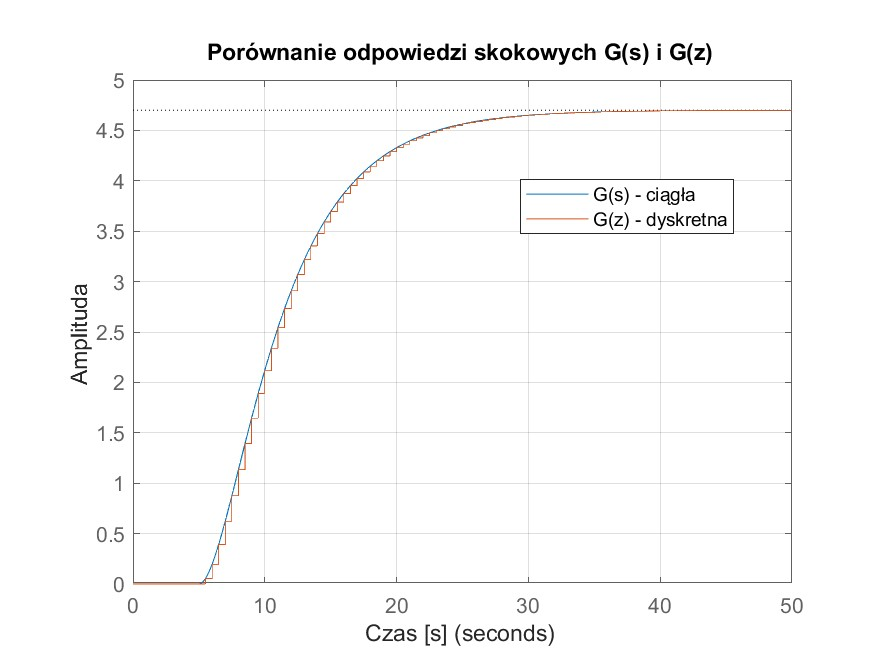
\includegraphics[width=0.8\textwidth]{kod/wykresy/zad1.jpg}
    \caption{Porównanie odpowiedzi skokowych obiektu ciągłego $G(s)$ i~dyskretnego $G(z)$ dla okresu próbkowania $T_p = 0,5$ s}
    \label{fig:odp_skokowe}
\end{figure}

Na rysunku \ref{fig:odp_skokowe} widać, że odpowiedzi skokowe modelu ciągłego i~dyskretnego są zbliżone, co potwierdza poprawność dyskretyzacji.

\section{Wyprowadzenie równania różnicowego}

Na podstawie transmitancji dyskretnej $G(z)$ wyprowadzono równanie różnicowe opisujące obiekt. Transmitancja dyskretna ma postać:
\begin{equation}
    G(z) = z^{-10} \cdot \frac{0,05477z + 0,04856}{z^2 - 1,675z + 0,6968}
\end{equation}

Równanie różnicowe wyprowadzone z~tej transmitancji:
\begin{equation}
    y(k) = 1,6748 \cdot y(k-1) - 0,69682 \cdot y(k-2) + 0,054771 \cdot u(k-11) + 0,048559 \cdot u(k-12)
\end{equation}

Ta postać pozwala na rekurencyjne obliczanie wyjścia procesu na podstawie poprzednich wartości wyjścia i~sterowania. Opóźnienie transportowe jest reprezentowane przez przesunięcie sygnału wejściowego o~10 okresów próbkowania ($u(k-10)$ i~później).

\section{Strojenie regulatora PID metodą Zieglera-Nicholsa}

Regulator PID został dostrojony metodą Zieglera-Nicholsa z~wykorzystaniem parametrów krytycznych. Na podstawie analizy charakterystyki częstotliwościowej obiektu wyznaczono następujące parametry krytyczne:
\begin{itemize}
    \item Wzmocnienie krytyczne $K_k = 0,46514$
    \item Okres oscylacji krytycznych $T_k = 10,6074$ s
    \item Pulsacja krytyczna $\omega_k = 0,59234$ rad/s
\end{itemize}

Zgodnie z~zasadami Zieglera-Nicholsa, obliczono parametry ciągłego regulatora PID:
\begin{itemize}
    \item $K_r = 0,16745$ (współczynnik wzmocnienia)
    \item $T_i = 8,8395$ s (stała czasowa całkowania)
    \item $T_d = 0,76373$ s (stała czasowa różniczkowania)
\end{itemize}

Co odpowiada następującym współczynnikom $K_p$, $K_i$ i~$K_d$:
\begin{itemize}
    \item $K_p = 0,16745$ (wzmocnienie członu proporcjonalnego)
    \item $K_i = 0,018943$ (wzmocnienie członu całkującego)
    \item $K_d = 0,12789$ (wzmocnienie członu różniczkującego)
\end{itemize}

Na podstawie tych wartości wyznaczono parametry dyskretnego regulatora PID w~postaci równania różnicowego:
\begin{equation}
    u(k) = u(k-1) + r_0 e(k) + r_1 e(k-1) + r_2 e(k-2)
\end{equation}

gdzie:
\begin{itemize}
    \item $r_0 = 0,4327$
    \item $r_1 = -0,679$
    \item $r_2 = 0,25577$
\end{itemize}

System wyświetlił ostrzeżenie, że układ zamknięty z~otrzymanymi parametrami może być niestabilny, co wskazuje na trudności w~regulacji tego obiektu przy użyciu standardowego regulatora PID. Jest to typowe dla obiektów z~dużym opóźnieniem transportowym.

\section{Synteza i~badanie regulatora DMC}

\subsection{Wyznaczenie horyzontu dynamiki}

Pierwszym krokiem w~syntezie regulatora DMC było wyznaczenie horyzontu dynamiki $D$, czyli liczby współczynników odpowiedzi skokowej koniecznych do poprawnego zamodelowania dynamiki obiektu. Na podstawie odpowiedzi skokowej obiektu (rysunek \ref{fig:step}) przyjęto $D = 60$, co odpowiada czasowi $30$ sekund (przy $T_p = 0,5$ s), po którym odpowiedź skokowa praktycznie osiąga stan ustalony.

\begin{figure}[H]
    \centering
    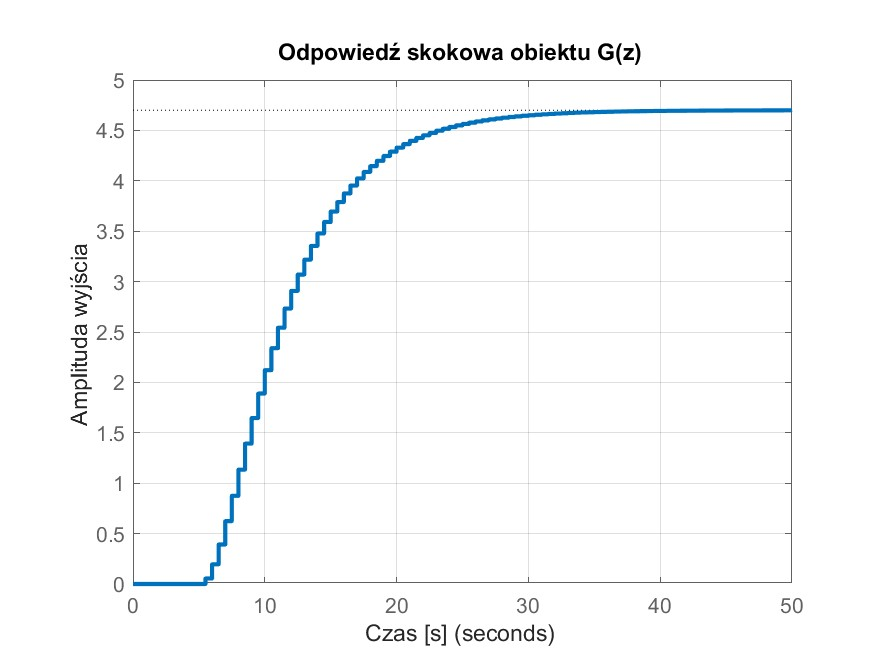
\includegraphics[width=0.7\textwidth]{kod/wykresy/step.jpg}
    \caption{Odpowiedź skokowa obiektu dyskretnego wykorzystana do wyznaczenia horyzontu dynamiki $D$}
    \label{fig:step}
\end{figure}

\subsection{Badanie wpływu horyzontu predykcji $N$}

W regulatorze DMC horyzont predykcji $N$ określa, na ile kroków w~przyszłość prognozowane jest zachowanie obiektu. Aby zbadać wpływ tego parametru na jakość regulacji, przeprowadzono symulację dla różnych wartości $N$ przy ustalonych pozostałych parametrach. Na rysunku \ref{fig:N_comparison} przedstawiono porównanie odpowiedzi układu dla wartości $N \in \{20, 30, 40, 50, 60\}$, przy założeniu $N_u = N$ i~$\lambda = 1$.

\begin{figure}[H]
    \centering
    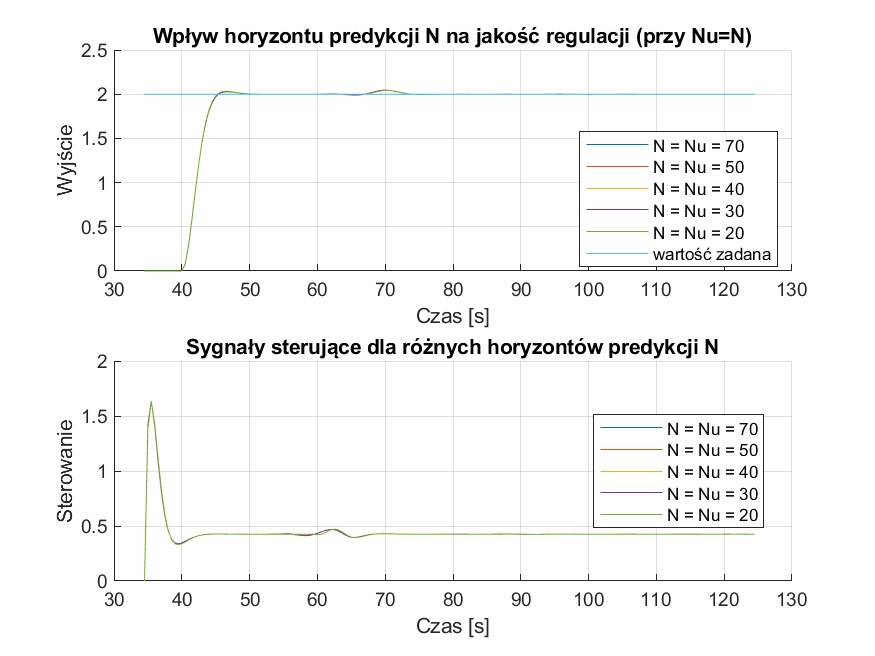
\includegraphics[width=0.8\textwidth]{kod/wykresy/horyzont_predykcji_porownanie.jpg}
    \caption{Wpływ horyzontu predykcji $N$ na jakość regulacji (przy $N_u = N$)}
    \label{fig:N_comparison}
\end{figure}

Z~analizy wynika, że dla $N < 30$ układ wykazuje słabsze tłumienie oscylacji. Przy większych wartościach odpowiedzi stają się bardziej stabilne, ale przy $N > 40$ dalsze zwiększanie horyzontu predykcji nie przynosi już znaczącej poprawy. Jako optymalną wybrano wartość $N = 20$.

\subsection{Badanie wpływu horyzontu sterowania $N_u$}

Horyzont sterowania $N_u$ określa, na ile kroków w~przyszłość obliczane są przyrosty sterowania. Aby zbadać wpływ tego parametru, przeprowadzono symulacje dla stałego horyzontu predykcji $N = 20$ i~różnych wartości $N_u \in \{1, 5, 10, 20, 40, 60\}$.

\begin{figure}[H]
    \centering
    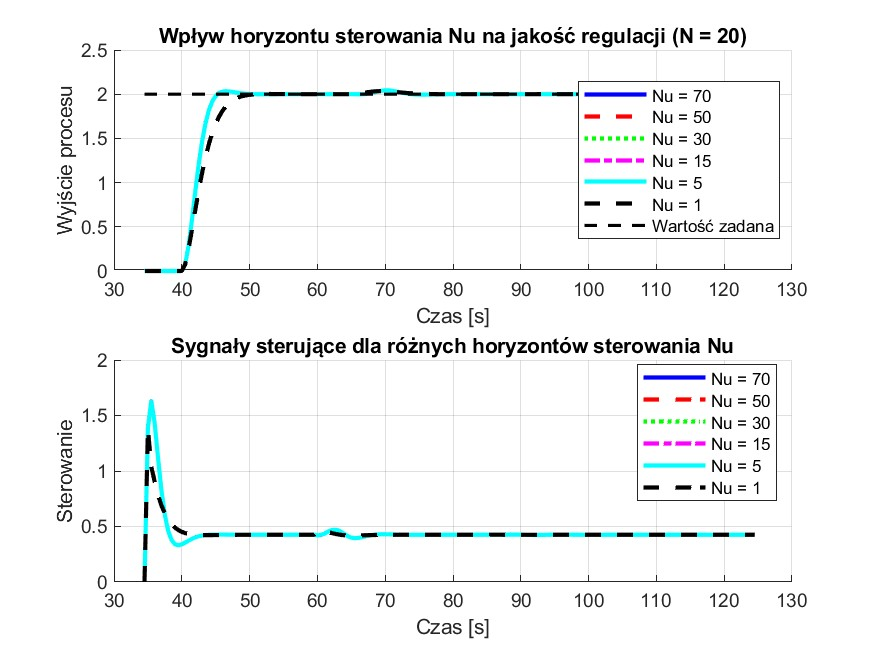
\includegraphics[width=0.8\textwidth]{kod/wykresy/horyzont_sterowania_porownanie.jpg}
    \caption{Wpływ horyzontu sterowania $N_u$ na jakość regulacji (przy $N = 20$)}
    \label{fig:Nu_comparison}
\end{figure}

Z~rysunku \ref{fig:Nu_comparison} wynika, że dla małych wartości $N_u$ (szczególnie $N_u = 1$) odpowiedź układu jest wolniejsza, ale za to łagodniejsza. Wraz ze wzrostem $N_u$ odpowiedź staje się szybsza, ale pojawia się przesterowanie i~większe oscylacje sterowania. Jako kompromis między szybkością a~jakością wybrano $N_u = 5$.

\subsection{Badanie wpływu współczynnika kary za sterowanie $\lambda$}

Współczynnik $\lambda$ odpowiada za wagę członu kary za przyrosty sterowania w~funkcji celu regulatora DMC. Im większa wartość $\lambda$, tym większa kara za duże zmiany sterowania, co prowadzi do łagodniejszego działania regulatora.

\begin{figure}[H]
    \centering
    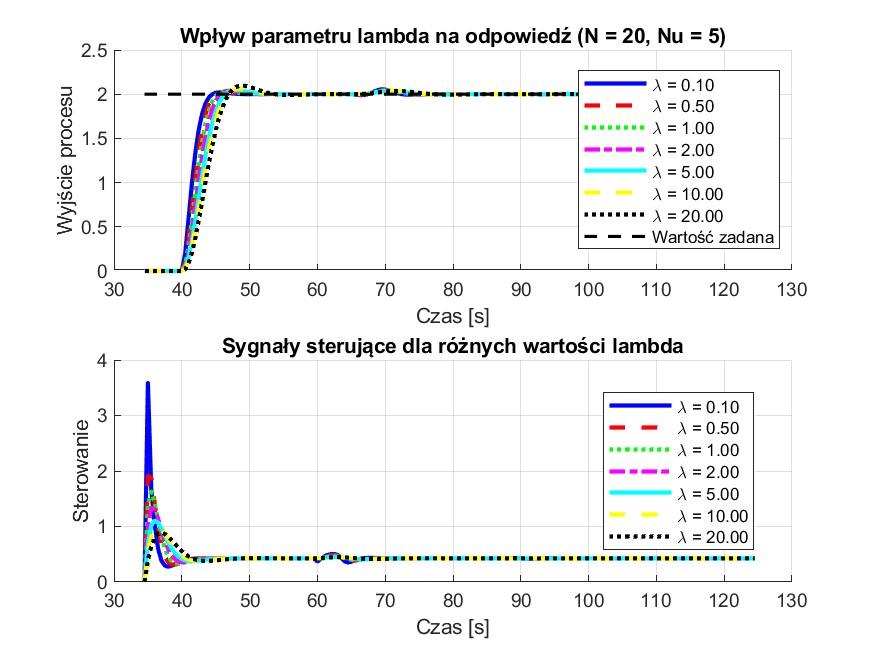
\includegraphics[width=0.8\textwidth]{kod/wykresy/lambda_porownanie.jpg}
    \caption{Wpływ współczynnika kary $\lambda$ na jakość regulacji (przy $N = 20$, $N_u = 5$)}
    \label{fig:lambda_comparison}
\end{figure}

Z~rysunku \ref{fig:lambda_comparison} wynika, że dla małych wartości $\lambda$ (np. $0,1$) układ reaguje szybko, ale sterowanie może być agresywne. Dla większych wartości $\lambda$ (np. $5$ czy $10$) odpowiedź jest wolniejsza i~łagodniejsza. Po przeprowadzeniu badań jako optymalną wartość wybrano $\lambda = 0,5$, która zapewnia dobry kompromis między szybkością odpowiedzi a~łagodnością profilu sterowania.

Po przeprowadzeniu powyższych badań ustalono optymalne parametry regulatora DMC:
\begin{itemize}
    \item Horyzont predykcji $N = 20$
    \item Horyzont sterowania $N_u = 5$
    \item Współczynnik kary $\lambda = 0,5$
\end{itemize}

\section{Porównanie regulatorów DMC i~PID}

Po określeniu optymalnych parametrów regulatora DMC przeprowadzono porównanie jego działania z~regulatorem PID dostrojonym metodą Zieglera-Nicholsa. Rysunek \ref{fig:dmc_pid} przedstawia porównanie odpowiedzi układu oraz sygnałów sterujących dla obu regulatorów.

\begin{figure}[H]
    \centering
    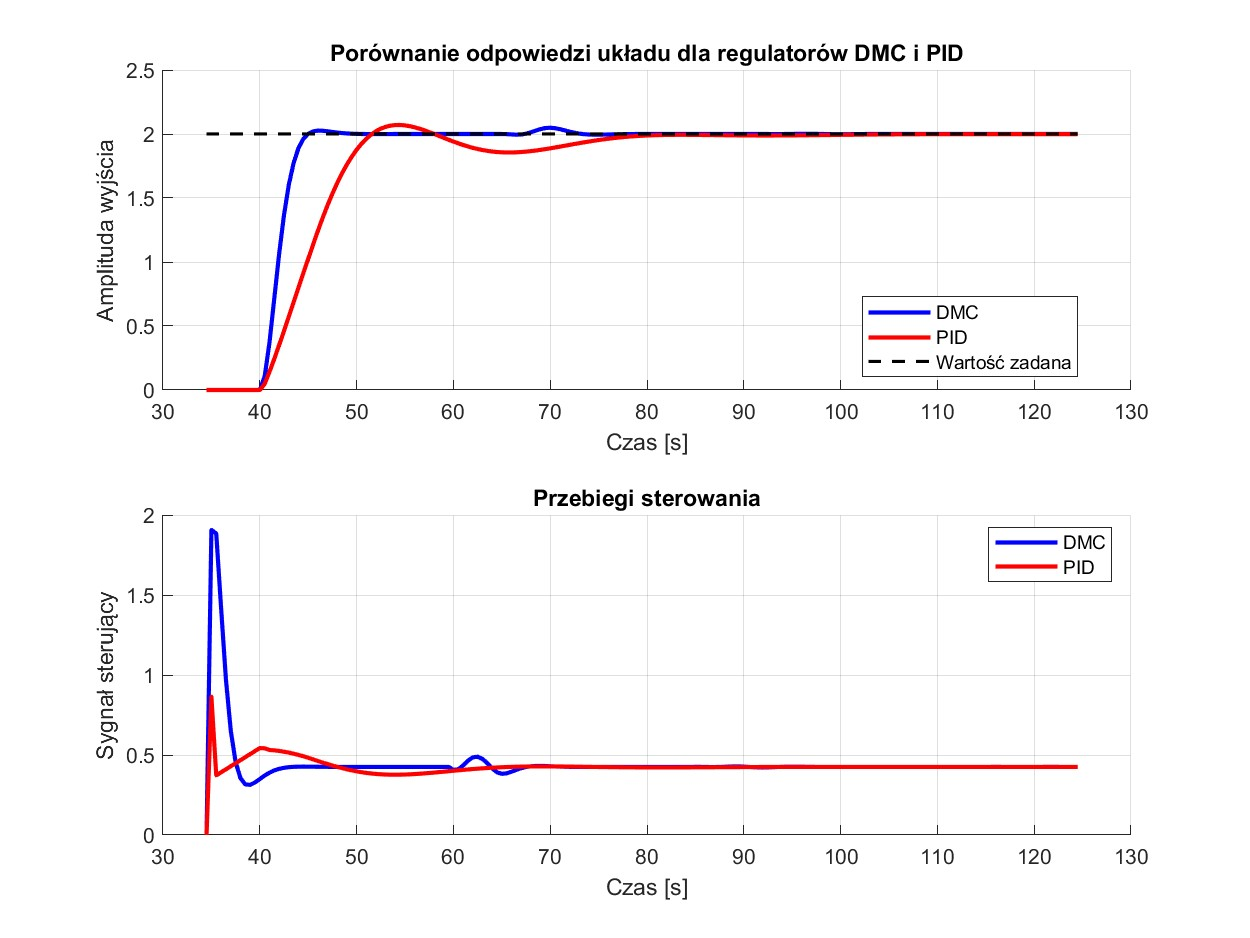
\includegraphics[width=0.8\textwidth]{kod/wykresy/optimal_solution.jpg}
    \caption{Porównanie odpowiedzi układu z~regulatorem DMC i~PID}
    \label{fig:dmc_pid}
\end{figure}

Regulator DMC wykazuje lepszą jakość regulacji niż PID - charakteryzuje się mniejszym przeregulowaniem, szybszym czasem regulacji i~lepszym tłumieniem oscylacji. Sygnał sterujący generowany przez DMC ma łagodniejszy przebieg niż w~przypadku PID, co jest korzystne z~punktu widzenia elementów wykonawczych.

\section{Porównanie regulatorów DMC i~GPC}

\subsection{Reakcja na zmianę wartości zadanej}

Porównano działanie regulatorów DMC i~GPC przy jednakowych parametrach ($N = 20$, $N_u = 5$, $\lambda = 0,1$). Na rysunku \ref{fig:dmc_gpc_setpoint} przedstawiono odpowiedź układu na zmianę wartości zadanej.

\begin{figure}[H]
    \centering
    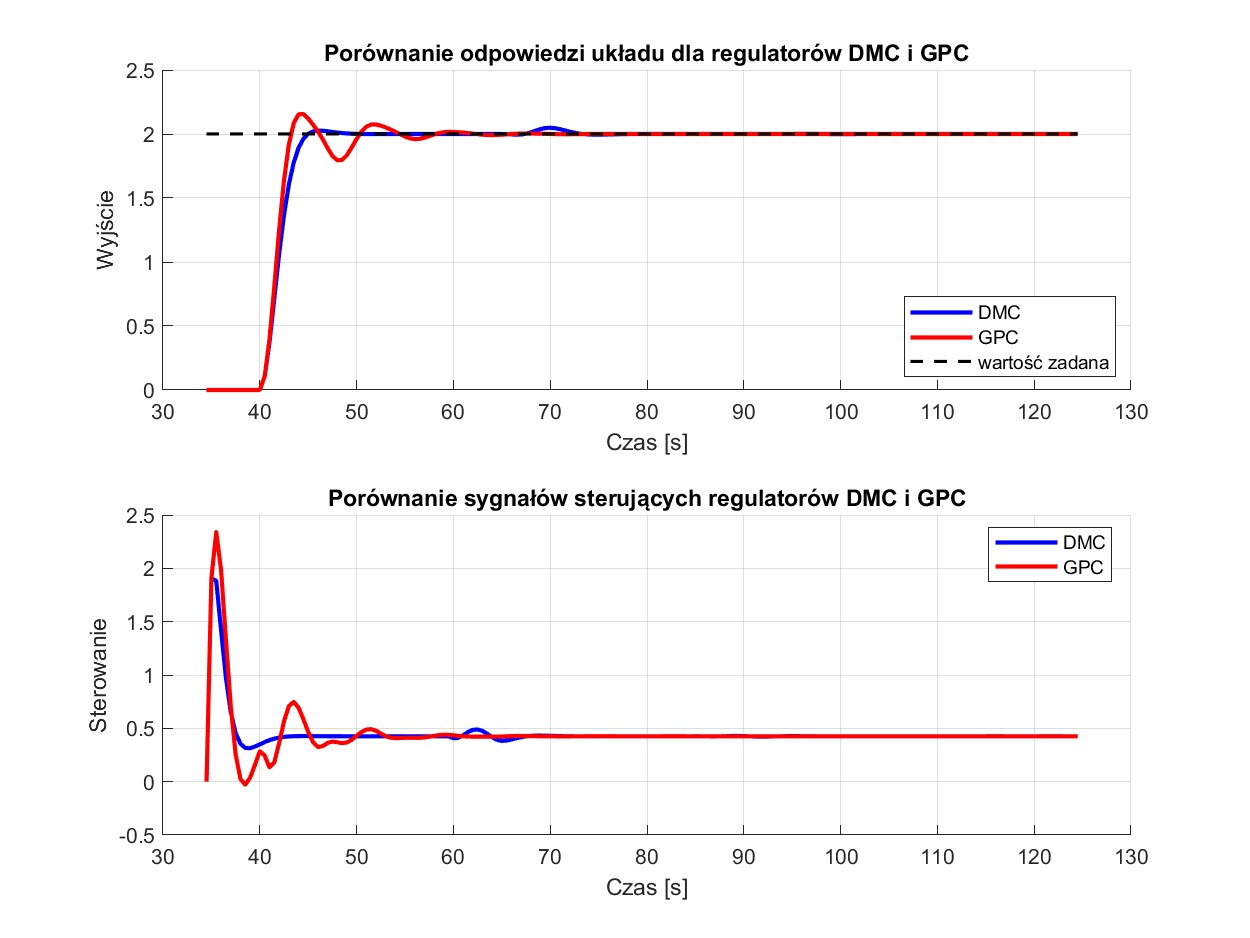
\includegraphics[width=0.8\textwidth]{kod/wykresy/DMC_vs_GPC_setpoint.jpg}
    \caption{Porównanie odpowiedzi układu z~regulatorami DMC i~GPC na zmianę wartości zadanej}
    \label{fig:dmc_gpc_setpoint}
\end{figure}

Zarówno regulator DMC, jak i~GPC zapewniają podobną jakość regulacji, jednak GPC charakteryzuje się nieco szybszą odpowiedzią i~mniejszym przeregulowaniem. Wynika to z~różnego sposobu modelowania obiektu w~tych algorytmach - DMC wykorzystuje model odpowiedzi skokowej, a~GPC - model w~postaci równania różnicowego.

\subsection{Reakcja na zakłócenie}

Przeprowadzono również test odporności na zakłócenie działające na wyjściu obiektu. Na rysunku \ref{fig:dmc_gpc_disturbance} przedstawiono odpowiedź układu na zakłócenie o~wartości $0,3$.

\begin{figure}[H]
    \centering
    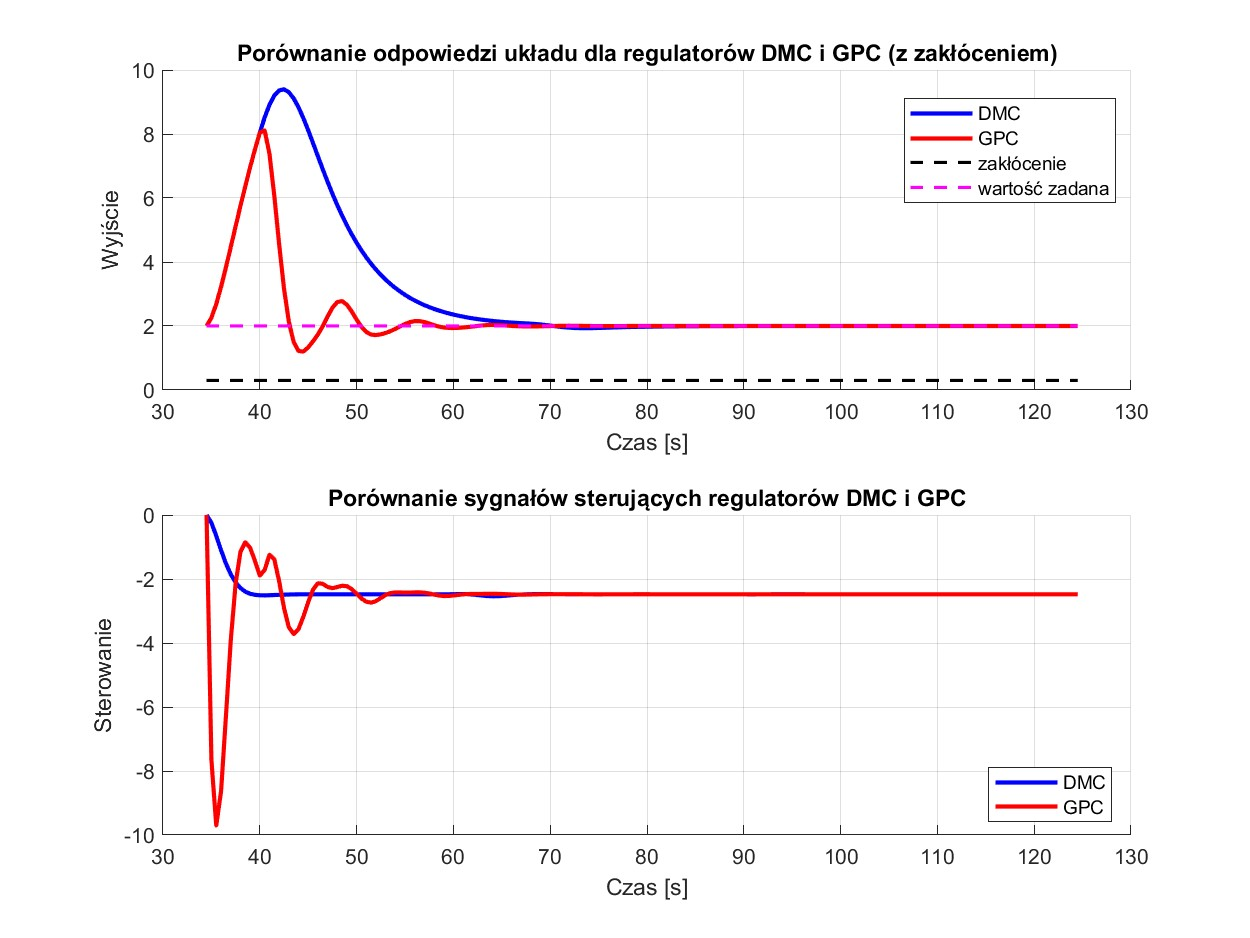
\includegraphics[width=0.8\textwidth]{kod/wykresy/DMC_vs_GPC_disturbance.jpg}
    \caption{Porównanie odpowiedzi układu z~regulatorami DMC i~GPC na zakłócenie}
    \label{fig:dmc_gpc_disturbance}
\end{figure}

W przypadku zakłócenia regulator GPC wykazuje szybszą reakcję i~lepsze tłumienie jego wpływu. Regulator DMC również skutecznie kompensuje zakłócenie, ale potrzebuje nieco więcej czasu. Wynika to z~różnych modeli procesu i~algorytmu predykcji zakłóceń.

\section{Badanie obszarów stabilności}

W ostatnim etapie projektu przeprowadzono badanie obszarów stabilności regulatorów PID, DMC i~GPC w~funkcji zmiany parametrów obiektu: wzmocnienia $K_o$ i~opóźnienia transportowego $T_o$. Zbadano wartości krytyczne wzmocnienia $K_o$ dla różnych wartości opóźnienia $T_o$, przy których układ regulacji traci stabilność.

Wyniki symulacji:
\begin{itemize}
    \item To=5,00, Ko\_kryt: GPC=41,20, DMC=30,50, PID=12,50
    \item To=5,50, Ko\_kryt: GPC=41,40, DMC=30,70, PID=11,60
    \item To=6,00, Ko\_kryt: GPC=43,30, DMC=31,00, PID=10,90
    \item To=6,50, Ko\_kryt: GPC=49,00, DMC=31,30, PID=10,70
    \item To=7,00, Ko\_kryt: GPC=70,70, DMC=30,50, PID=10,10
    \item To=7,50, Ko\_kryt: GPC=68,00, DMC=31,90, PID=9,60
    \item To=8,00, Ko\_kryt: GPC=97,70, DMC=35,00, PID=9,10
    \item To=8,50, Ko\_kryt: GPC=5,70, DMC=27,90, PID=8,70
    \item To=9,00, Ko\_kryt: GPC=9,40, DMC=47,90, PID=8,50
    \item To=9,50, Ko\_kryt: GPC=0,00, DMC=0,00, PID=8,80
    \item To=10,00, Ko\_kryt: GPC=0,00, DMC=0,00, PID=8,40
\end{itemize}

Na rysunku \ref{fig:stability} przedstawiono otrzymane krzywe graniczne stabilności.

\begin{figure}[H]
    \centering
    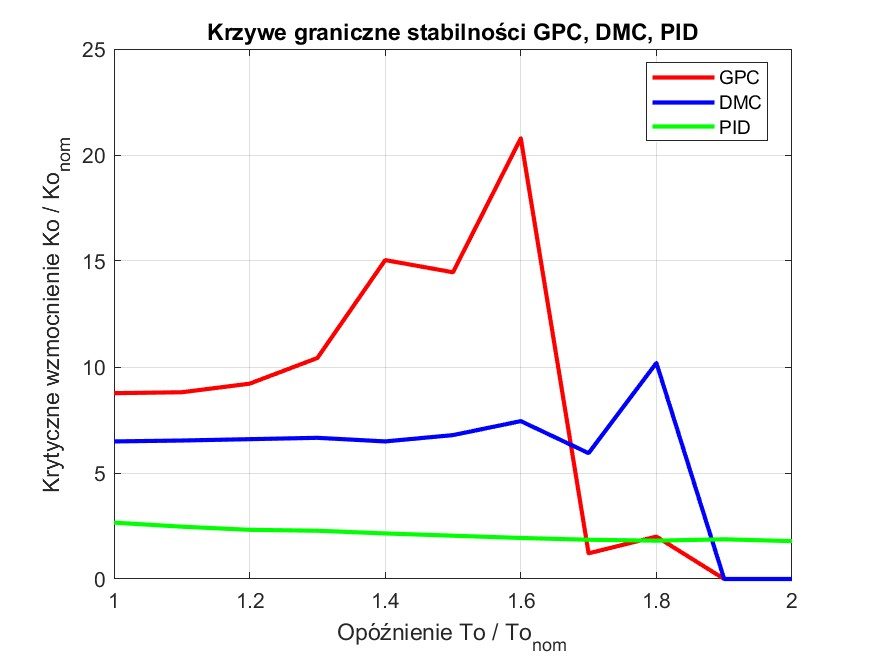
\includegraphics[width=0.8\textwidth]{kod/wykresy/GPC_DMC_PID_stabilnosc_Ko_vs_To.jpg}
    \caption{Krzywe graniczne stabilności dla regulatorów GPC, DMC i~PID w~funkcji opóźnienia $T_o$ i~wzmocnienia $K_o$}
    \label{fig:stability}
\end{figure}

Na osiach wykresu przedstawiono względne zmiany parametrów $T_o/T_{o,nom}$ oraz $K_o/K_{o,nom}$. Obszar stabilności leży poniżej krzywych dla każdego z~regulatorów - dla danego opóźnienia $T_o/T_{o,nom}$, system jest stabilny jeśli $K_o/K_{o,nom} < K_{o,kryt}/K_{o,nom}$.

Widoczne jest, że regulatory predykcyjne (DMC i~GPC) mają znacznie szerszy obszar stabilności niż regulator PID, szczególnie dla większych opóźnień. Regulator GPC wykazuje największą odporność na wzrost opóźnienia transportowego, co jest jego istotną zaletą w~zastosowaniach przemysłowych, zgodnie z~teorią regulacji predykcyjnej.

Warto odnotować, że dla bardzo dużych opóźnień (To > 9,0) wszystkie regulatory tracą stabilność nawet przy niewielkim wzroście wzmocnienia obiektu. Jest to zgodne z~teorią sterowania, ponieważ duże opóźnienie transportowe jest jednym z~najtrudniejszych wyzwań w~regulacji.

\chapter{Wnioski}

Na podstawie przeprowadzonych badań można sformułować następujące wnioski:

\begin{enumerate}
    \item Regulatory predykcyjne (DMC i~GPC) zapewniają lepszą jakość regulacji niż klasyczny regulator PID, szczególnie dla obiektów z~opóźnieniem transportowym. Wykazują mniejsze przeregulowanie, krótszy czas regulacji i~lepsze tłumienie oscylacji.

    \item Parametry regulatora DMC ($N$, $N_u$, $\lambda$) mają istotny wpływ na jakość regulacji. Horyzont predykcji $N$ powinien być wystarczająco duży, aby uwzględnić pełną odpowiedź obiektu. Horyzont sterowania $N_u$ wpływa na agresywność sterowania - większe wartości prowadzą do szybszej, ale bardziej oscylacyjnej odpowiedzi. Współczynnik $\lambda$ pozwala na kompromis między szybkością regulacji a~łagodnością sterowania.

    \item Regulator GPC wykazuje lepsze właściwości niż DMC w~zakresie kompensacji zakłóceń oraz odporności na zmiany parametrów obiektu, szczególnie opóźnienia transportowego. Wynika to z~odmiennego sposobu modelowania obiektu i~predykcji - GPC wykorzystuje model w~postaci równania różnicowego, co pozwala na dokładniejsze odzwierciedlenie dynamiki systemu.

    \item Obszar stabilności regulatorów predykcyjnych jest znacznie szerszy niż regulatora PID, co czyni je bardziej odpornymi na zmiany parametrów obiektu. Jest to szczególnie istotne w~przypadku procesów o~zmiennych parametrach lub niepewności modelowania.
\end{enumerate}

Podsumowując, regulatory predykcyjne stanowią efektywne narzędzie do sterowania procesami, szczególnie w~przypadku obiektów trudnych (z opóźnieniem, niestabilnych, wielowymiarowych). Ich implementacja wymaga jednak dokładniejszego modelowania procesu oraz większej mocy obliczeniowej niż w~przypadku klasycznych regulatorów PID.

\chapter{Kod źródłowy}

Poniżej przedstawiono listę skryptów MATLAB wykorzystanych w projekcie. Szczegółowe treści tych skryptów znajdują się w katalogu \texttt{/home/jszubzda/STP\_2/kod/}.

\section{Główny skrypt projektu}

\lstinputlisting[style=custommatlab, caption={Główny skrypt projektu - stp2.m}, label={lst:main}]{kod/stp2.m}

\section{Funkcje do analizy transmitancji i wyprowadzenia równania różnicowego}

\lstinputlisting[style=custommatlab, caption={zadanie1\_analiza\_transmitancji.m}, label={lst:zadanie1}]{kod/zadanie1_analiza_transmitancji.m}

\lstinputlisting[style=custommatlab, caption={zadanie2\_rownanie\_roznicowe.m}, label={lst:zadanie2}]{kod/zadanie2_rownanie_roznicowe.m}

\section{Funkcje do strojenia regulatora PID}

\lstinputlisting[style=custommatlab, caption={zadanie3\_strojenie\_pid\_ziegler\_nichols.m}, label={lst:zadanie3}]{kod/zadanie3_strojenie_pid_ziegler_nichols.m}

\section{Funkcje do projektowania i badania regulatora DMC}

\lstinputlisting[style=custommatlab, caption={zadanie5\_optymalizacja\_dmc.m}, label={lst:zadanie5}]{kod/zadanie5_optymalizacja_dmc.m}

\lstinputlisting[style=custommatlab, caption={zadanie6\_porownanie\_optymalne\_dmc\_pid.m}, label={lst:zadanie6}]{kod/zadanie6_porownanie_optymalne_dmc_pid.m}

\section{Funkcje do porównania regulatorów DMC i GPC}

\lstinputlisting[style=custommatlab, caption={zadanie8\_porownanie\_dmc\_gpc.m}, label={lst:zadanie8}]{kod/zadanie8_porownanie_dmc_gpc.m}

\section{Funkcje do badania stabilności}

\lstinputlisting[style=custommatlab, caption={zadanie9\_badanie\_stabilnosci.m}, label={lst:zadanie9}]{kod/zadanie9_badanie_stabilnosci.m}

\lstinputlisting[style=custommatlab, caption={czy\_oscyluje.m}, label={lst:czy_oscyluje}]{kod/czy_oscyluje.m}

\section{Funkcje pomocnicze do symulacji}

\lstinputlisting[style=custommatlab, caption={symulacja\_dmc\_pid.m}, label={lst:symulacja_dmc_pid}]{kod/symulacja_dmc_pid.m}

\lstinputlisting[style=custommatlab, caption={symulacja\_gpc.m}, label={lst:symulacja_gpc}]{kod/symulacja_gpc.m}

\end{document}
